\section{Conclusiones y Trabajo Futuro}
\begin{frame}{Conclusiones}
    \begin{enumerate}
        \item<1-> El tamaño del CT calculado con el algoritmo ROCLOUD muestra ser operacionalmente funcional. Otros estudios similares no tienen en cuenta la precipitación del CT. 
        \\~\
        \item<2-> Además, la intensidad del CT no está relacionada con su tamaño. Por ejemplo, los TD pueden tener un tamaño mayor que los huracanes.
        \\~\
        \item<3-> La precipitación del CT calculada a partir de dos enfoques (radio de las bandas de lluvia del CT y perfiles pcp) muestra que los CT producen importantes precipitaciones en regiones remotas situadas a ~750 km del centro del CT. Es  mayor sobre las regiones continentales ya que las bandas de lluvia están más dispersas que sobre las regiones oceánicas.
    \end{enumerate}
\end{frame}

\begin{frame}{Conclusiones}
    \begin{enumerate}
    \setcounter{enumi}{3}
        \item<1->Las variables a gran escala desempeñan un papel importante en la determinación de las precipitaciones del CT.
        \\~\
        \item<2->La humedad a niveles medios, la cizalladura del viento y la divergencia en la atmósfera superior muestran una fuerte relación con la precipitación del CT. 
        \\~\
        \item<3->Finalmente, las métricas de forma Dispersión ($D$), Asimetría ($A$) y Solidez ($S$) muestran que, en promedio, los CTs de ambas cuencas tienden a ser más dispersos, asimétricos y menos sólidos.
    \end{enumerate}
\end{frame}

\begin{frame}
\begin{columns}
    \begin{column}{0.5\textwidth}
        \begin{block}{\textbf{Sobre el SIAT-CT}}
        La motivación principal de este trabajo radica en las limitaciones que tiene el SIAT-CT en términos de la definición del tamaño. Los resultados muestran que la influencia de la PCT puede alcanzar los 750 km desde el centro del CT. Por ello, se vuelve relevante usar una definición diferente al R34, que incorpore un tamaño del CT que considere la extensión de las bandas nubosas del CT y su precipitación.
        \end{block}
    \end{column}
    \begin{column}{0.5\textwidth}
    \begin{figure}
        \centering
        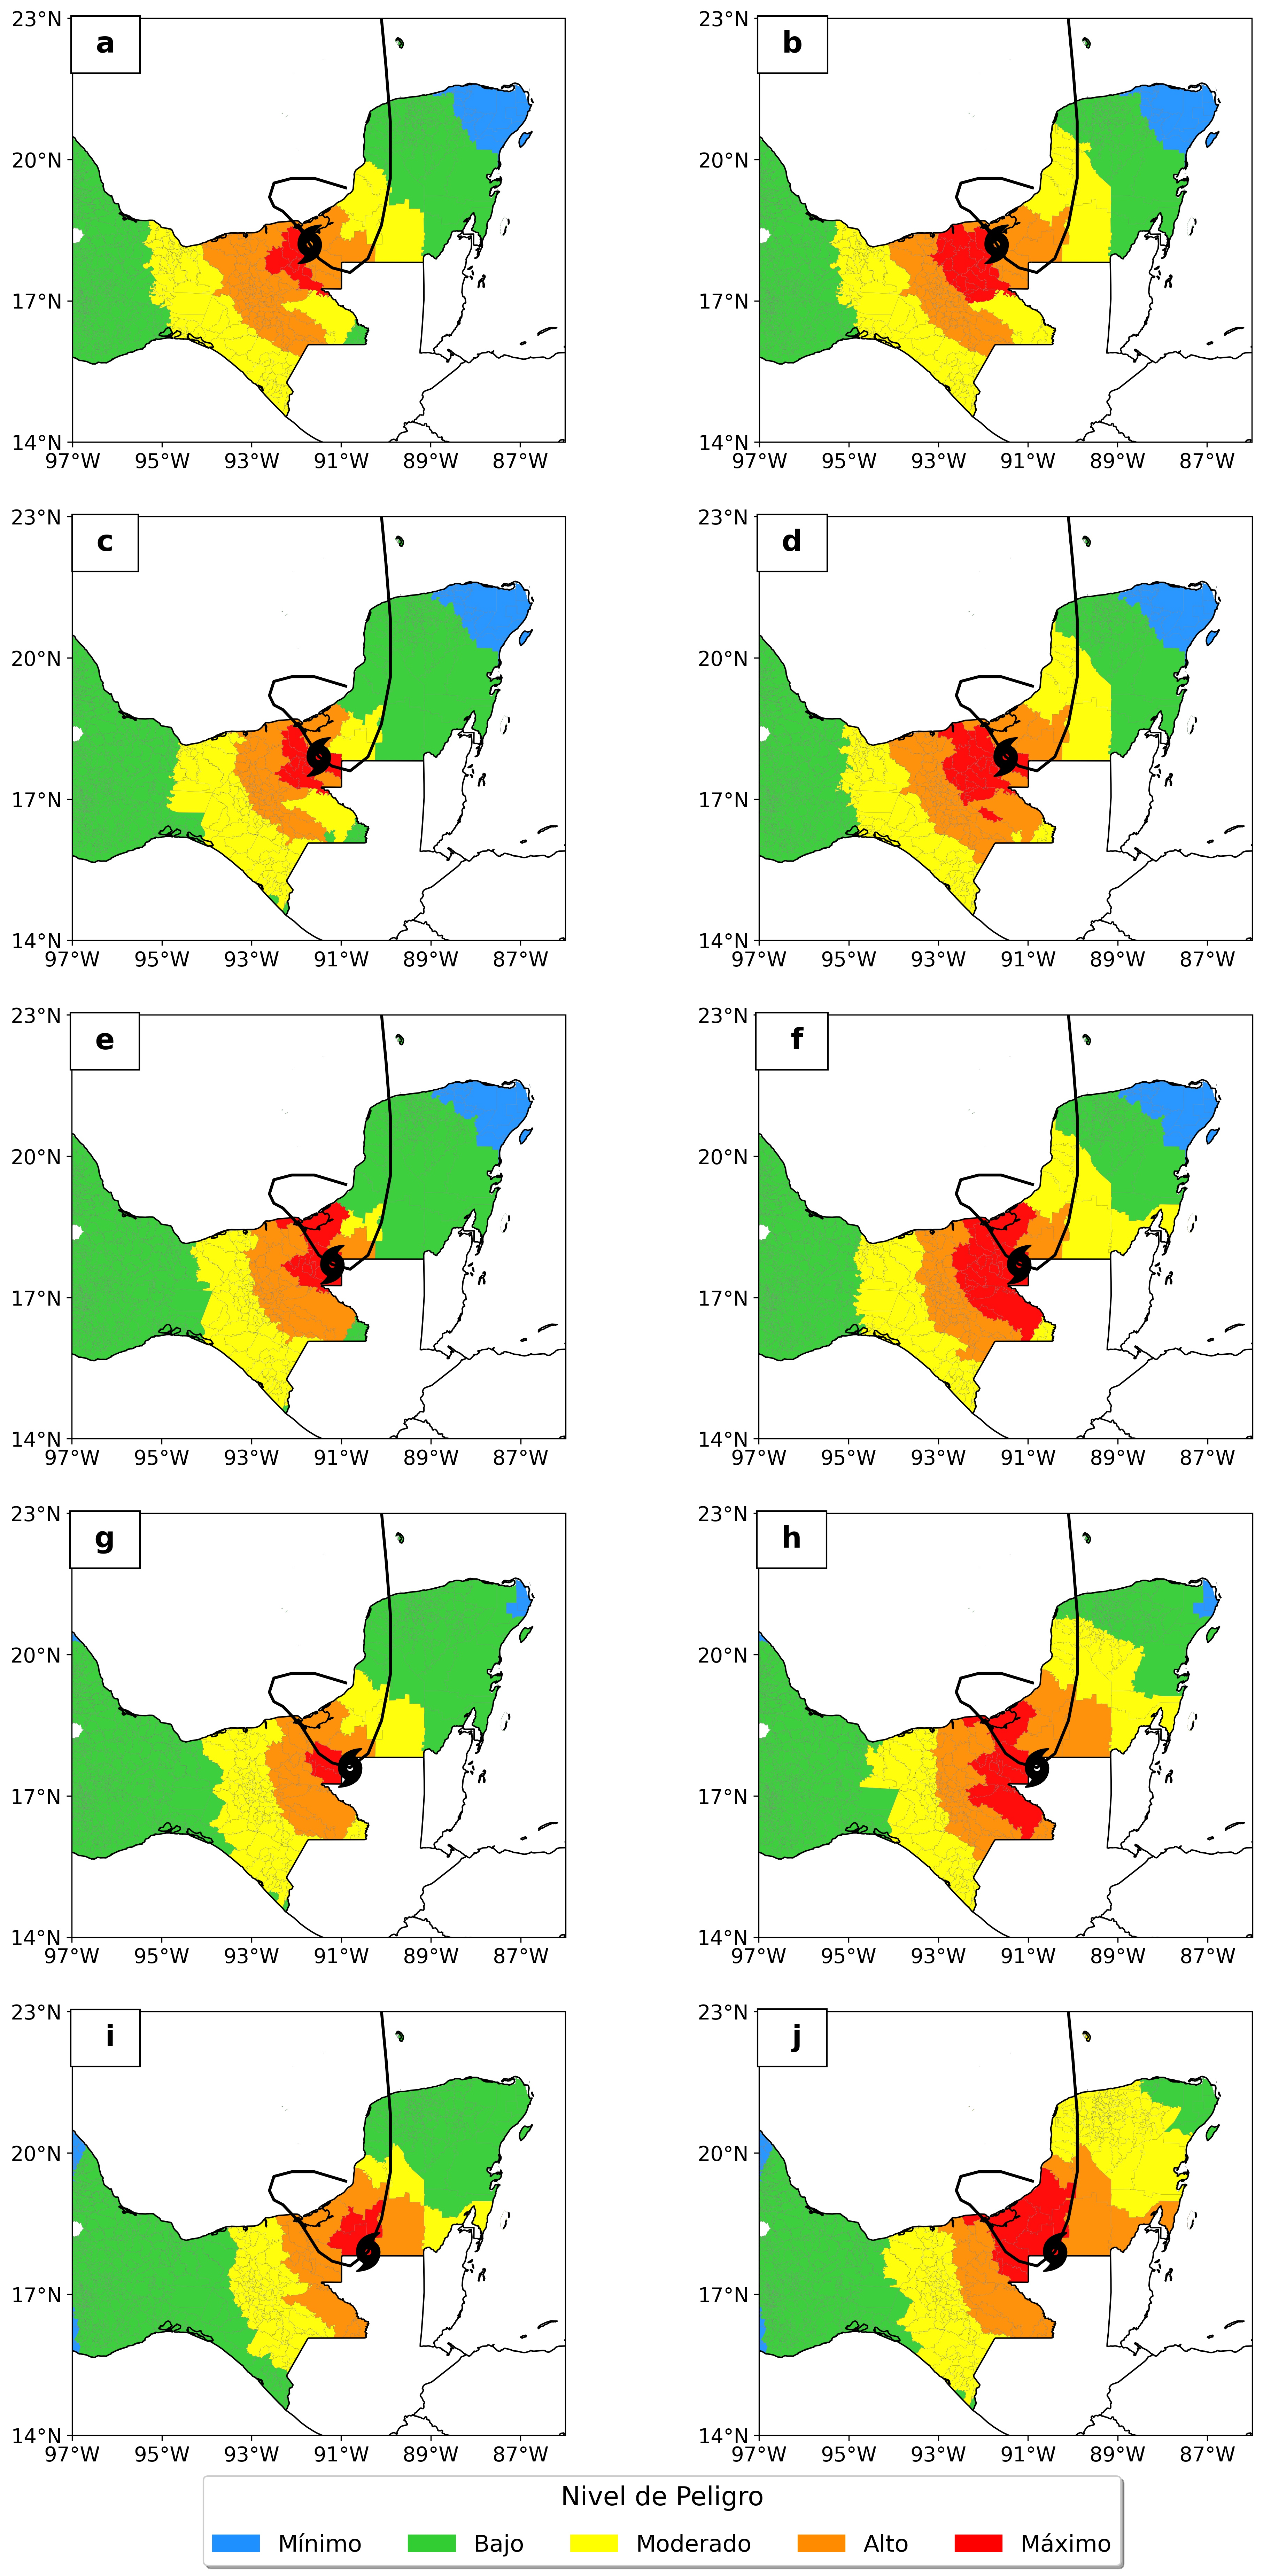
\includegraphics[scale = 0.135]{Images/Figures/Fig_4_1.jpeg}
        \label{fig:fig_conclusion}
    \end{figure}
    \end{column}
\end{columns}
\end{frame}

\begin{frame}{Trabajo Futuro}
    \begin{itemize}
        \item Estudiar posibles mejoras en las alertas tempranas modificando los tamaños del CT.
        \\~\
        \item Usar técnicas de machine learning para predecir el tamaño de un CT, con fines operativos.
        \\~\
        \item Estudiar el cambio climático y su papel en el tamaño de los CTs en un futuro.
    \end{itemize}
\end{frame}


% This section is a placeholder for you to go over crucial points to takeaway from your presentation.

\begin{frame}
\begin{center}
\Huge ¡Muchas Gracias!
\end{center}
\end{frame}